\documentclass[journal,12pt,twocolumn]{IEEEtran}

\usepackage{setspace}
\usepackage{gensymb}
\singlespacing
\usepackage[cmex10]{amsmath}

\usepackage{amsthm}

\usepackage{mathrsfs}
\usepackage{txfonts}
\usepackage{stfloats}
\usepackage{bm}
\usepackage{cite}
\usepackage{cases}
\usepackage{subfig}

\usepackage{longtable}
\usepackage{multirow}
\usepackage{graphicx}
\usepackage{enumitem}
\usepackage{mathtools}
\usepackage{steinmetz}
\usepackage{tikz}
\usepackage{circuitikz}
\usepackage{verbatim}
\usepackage{tfrupee}
\usepackage[breaklinks=true]{hyperref}
\usepackage{graphicx}
\usepackage{tkz-euclide}
\usepackage{amsmath}
\usetikzlibrary{calc,math}
\usepackage{listings}
    \usepackage{color}                                            %%
    \usepackage{array}                                            %%
    \usepackage{longtable}                                        %%
    \usepackage{calc}                                             %%
    \usepackage{multirow}                                         %%
    \usepackage{hhline}                                           %%
    \usepackage{ifthen}                                           %%
    \usepackage{lscape}     
\usepackage{multicol}
\usepackage{chngcntr}

\DeclareMathOperator*{\Res}{Res}

\renewcommand\thesection{\arabic{section}}
\renewcommand\thesubsection{\thesection.\arabic{subsection}}
\renewcommand\thesubsubsection{\thesubsection.\arabic{subsubsection}}

\renewcommand\thesectiondis{\arabic{section}}
\renewcommand\thesubsectiondis{\thesectiondis.\arabic{subsection}}
\renewcommand\thesubsubsectiondis{\thesubsectiondis.\arabic{subsubsection}}

\graphicspath{{figures/}}

\hyphenation{op-tical net-works semi-conduc-tor}
\def\inputGnumericTable{}                                 %%

\lstset{
%language=C,
frame=single, 
breaklines=true,
columns=fullflexible
}
\begin{document}


\newtheorem{theorem}{Theorem}[section]
\newtheorem{problem}{Problem}
\newtheorem{proposition}{Proposition}[section]
\newtheorem{lemma}{Lemma}[section]
\newtheorem{corollary}[theorem]{Corollary}
\newtheorem{example}{Example}[section]
\newtheorem{definition}[problem]{Definition}

\newcommand{\BEQA}{\begin{eqnarray}}
\newcommand{\EEQA}{\end{eqnarray}}
\newcommand{\define}{\stackrel{\triangle}{=}}
\bibliographystyle{IEEEtran}
\raggedbottom
\setlength{\parindent}{0pt}
\providecommand{\mbf}{\mathbf}
\providecommand{\pr}[1]{\ensuremath{\Pr\left(#1\right)}}
\providecommand{\qfunc}[1]{\ensuremath{Q\left(#1\right)}}
\providecommand{\sbrak}[1]{\ensuremath{{}\left[#1\right]}}
\providecommand{\lsbrak}[1]{\ensuremath{{}\left[#1\right.}}
\providecommand{\rsbrak}[1]{\ensuremath{{}\left.#1\right]}}
\providecommand{\brak}[1]{\ensuremath{\left(#1\right)}}
\providecommand{\lbrak}[1]{\ensuremath{\left(#1\right.}}
\providecommand{\rbrak}[1]{\ensuremath{\left.#1\right)}}
\providecommand{\cbrak}[1]{\ensuremath{\left\{#1\right\}}}
\providecommand{\lcbrak}[1]{\ensuremath{\left\{#1\right.}}
\providecommand{\rcbrak}[1]{\ensuremath{\left.#1\right\}}}
\theoremstyle{remark}
\newtheorem{rem}{Remark}
\newcommand{\sgn}{\mathop{\mathrm{sgn}}}
\providecommand{\abs}[1]{$\left\vert#1\right\vert$}
\providecommand{\res}[1]{\Res\displaylimits_{#1}} 
\providecommand{\norm}[1]{$\left\lVert#1\right\rVert$}
%\providecommand{\norm}[1]{\lVert#1\rVert}
\providecommand{\mtx}[1]{\mathbf{#1}}
\providecommand{\mean}[1]{E$\left[ #1 \right]$}
\providecommand{\fourier}{\overset{\mathcal{F}}{ \rightleftharpoons}}
%\providecommand{\hilbert}{\overset{\mathcal{H}}{ \rightleftharpoons}}
\providecommand{\system}{\overset{\mathcal{H}}{ \longleftrightarrow}}
	%\newcommand{\solution}[2]{\textbf{Solution:}{#1}}
\newcommand{\solution}{\noindent \textbf{Solution: }}
\newcommand{\cosec}{\,\text{cosec}\,}
\providecommand{\dec}[2]{\ensuremath{\overset{#1}{\underset{#2}{\gtrless}}}}
\newcommand{\myvec}[1]{\ensuremath{\begin{pmatrix}#1\end{pmatrix}}}
\newcommand{\mydet}[1]{\ensuremath{\begin{vmatrix}#1\end{vmatrix}}}
\numberwithin{equation}{subsection}
\makeatletter
\@addtoreset{figure}{problem}
\makeatother
\let\StandardTheFigure\thefigure
\let\vec\mathbf
\renewcommand{\thefigure}{\theproblem}
\def\putbox#1#2#3{\makebox[0in][l]{\makebox[#1][l]{}\raisebox{\baselineskip}[0in][0in]{\raisebox{#2}[0in][0in]{#3}}}}
     \def\rightbox#1{\makebox[0in][r]{#1}}
     \def\centbox#1{\makebox[0in]{#1}}
     \def\topbox#1{\raisebox{-\baselineskip}[0in][0in]{#1}}
     \def\midbox#1{\raisebox{-0.5\baselineskip}[0in][0in]{#1}}
\vspace{3cm}
\title{Assignment 4}
\author{Vaddamani Saketh - CS20BTECH11054}
\maketitle
\newpage
\bigskip
\renewcommand{\thefigure}{\theenumi}
\renewcommand{\thetable}{\theenumi}
Download all python codes from 
\begin{lstlisting}
https://github.com/CS20BTECH11054/AI1103/blob/main/Assignment_4/codes/Assignment_4.py
\end{lstlisting}
%
and latex-tikz codes from 
%
\begin{lstlisting}
https://github.com/CS20BTECH11054/AI1103/blob/main/Assignment_4/Assignment_4.tex
\end{lstlisting}
\section{Problem}
Let a random variable $X$ follow exponential distribution with mean 2. Define $Y=[X-2|X>2]$. The value of $\pr{Y \geq t}$ is

\section{Solution}
Given that, $Y=[X-2|X>2]$
\begin{align}
\pr{Y \geq t} = \frac{\pr{X-2 \geq t, X>2}}{\pr{X>2}} \label{Eq:1}
\end{align}
Let the PDF,CDF, and mean for the distribution be $f\brak{x}$, $F_X\brak{x}$ and $E\brak{x}$ such that
\begin{align}
f\brak{x} = \begin{cases} \label{Eq:2}
			\lambda e^{-\lambda x}, & \text{if $0 < x< \infty $}\\
            0, & \text{otherwise}
		 \end{cases} \\
F_X\brak{x} = \begin{cases} \label{Eq:3}
			1 - e^{-\lambda x}, & \text{if $0 < x< \infty $}\\
            0, & \text{otherwise}
		 \end{cases} \\
E\brak{x} = \frac{1}{\lambda} \label{Eq:4}
\end{align}
Given, the mean or expected value of the distribution is 2, So, from \eqref{Eq:4}, we get
\begin{align}
\frac{1}{\lambda} = 2 \notag \\
\lambda = \frac{1}{2} \label{Eq:5}
\end{align}
$\pr{X > 2}$ can be found by
\begin{align}
\pr{X >2} = 1- F_X\brak{2} = e^{-2\lambda} \label{Eq:7} 
\end{align}
There are two cases possible depending on the value of t, They are,
\begin{align}
\brak{i} t>0 \notag
\end{align}
\begin{align}
\brak{ii} t\leq 0 \notag
\end{align}
$\underline{Case-\brak{i}:}$ $t>0$
\begin{align}
\pr{X \geq t+2,X>2} = \pr{X \geq t+2} \label{Eq:6}
\end{align}
\eqref{Eq:6} can be explained by the fact that if $t>0$ and $X>2$, then $X>t+2$ is a superset of $X>2$.
\begin{align}
\pr{X \geq t+2} = \pr{X > t+2} = 1- F_X\brak{t+2} = e^{-\lambda \brak{t+2}}\label{Eq:8}
\end{align}
Substituting \eqref{Eq:6}, \eqref{Eq:7} and \eqref{Eq:8} in \eqref{Eq:1}, we get
\begin{align}
\pr{Y \geq t} = \frac{e^{-\lambda \brak{t+2}}}{e^{-2\lambda}} = e^{-\lambda t} = e^{-\frac{t}{2}}
\end{align}
$\underline{Case-\brak{ii}:}$ $t \leq 0$
\begin{align}
\pr{X \geq t+2,X>2} = \pr{X>2} \label{Eq:8}
\end{align}
\eqref{Eq:8} can be explained by the fact that if $t\leq 0$ and $X \geq t+2$, then $X>2$ is a superset of $X\geq t+2$.  Substituting \eqref{Eq:8} in \eqref{Eq:1}, we get
\begin{align}
\pr{Y \geq t} = \frac{\pr{X>2}}{\pr{X>2}} = 1
\end{align}
Therefore, 
\begin{align}
 \pr{Y \geq t} =  \begin{cases}
			e^{-\frac{t}{2}}, & \text{if $t>0$}\\
            1, & \text{otherwise}
		 \end{cases} 
\end{align}
\newpage
\begin{figure}
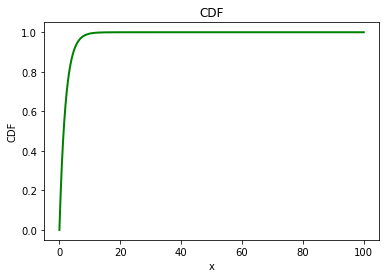
\includegraphics[width=\columnwidth]{figure_1.png}
    \caption{\textbf{\huge{CDF}}} 
\end{figure}
\begin{figure}
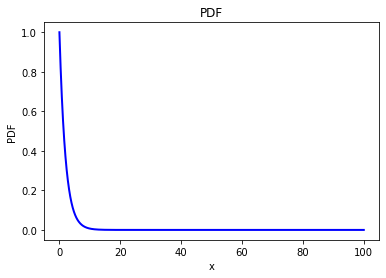
\includegraphics[width=\columnwidth]{figure_2.png}
    \caption{\textbf{\huge{PDF}}}
\end{figure}
\end{document}

 